\documentclass{article}
\title{Mapping randomly generated short \textit{k}-mers to genomes}
\author{Dave Tang  \\
	RIKEN Yokohama \\
        \href{https://twitter.com/davetang31}{@davetang31} \\
	\and 
	Derek de Rie \\
	VU University Amsterdam \\
        \href{https://twitter.com/derekderie}{@derekderie} \\
	}

\date{\today}

\usepackage{graphicx}
\graphicspath{ {image/} }
\usepackage{caption}
\usepackage{subcaption}
\usepackage{epstopdf}

\usepackage[english]{babel}
\usepackage{blindtext}

\usepackage{hyperref}
\hypersetup{
   colorlinks,
   citecolor=black,
   filecolor=black,
   linkcolor=black,
   urlcolor=black
}

\begin{document}

\maketitle

\begin{abstract}

Eukaryote genomes are composed of genic and non-genic stretches of DNA and depending on the organism, the ratio between the two are extremely variable. For example, the completion of the human genome revealed that only 1-2\% of the human genome is made up on protein-coding genes and the rest is composed of non-coding DNA. The portion of non-coding DNA is largely made up of repetitive elements, such as transposons and satellite repeats.

Despite their size, microRNAs (miRNAs) can have dramatic effects on human health due to their direct effect on transcripts. The misregulation of miRNAs can cause a wide spectrum of diseases, such as cancer, and as such they are under heavily investigation.

\end{abstract}

\section{Introduction}
MicroRNAs (miRNAs) were discovered in 1993\cite{pmid8252621} and are the most well known class of non-coding RNAs (ncRNAs). Since its discovery, \emph{miRBase}, a widely used database of miRNA annotations, has accumulated nearly 25,000 miRNA loci in over 200 species. The flood in annotations has been paired with an extensive amount of literature published on miRNA. In the nearly 15 years since the definition of a miRNA was introduced, NCBI's PubMed has collected over 30,000 publications containing the term microRNA (Figure ~\ref{fig:mirna_history}).

\begin{figure}[t]
   \centering
      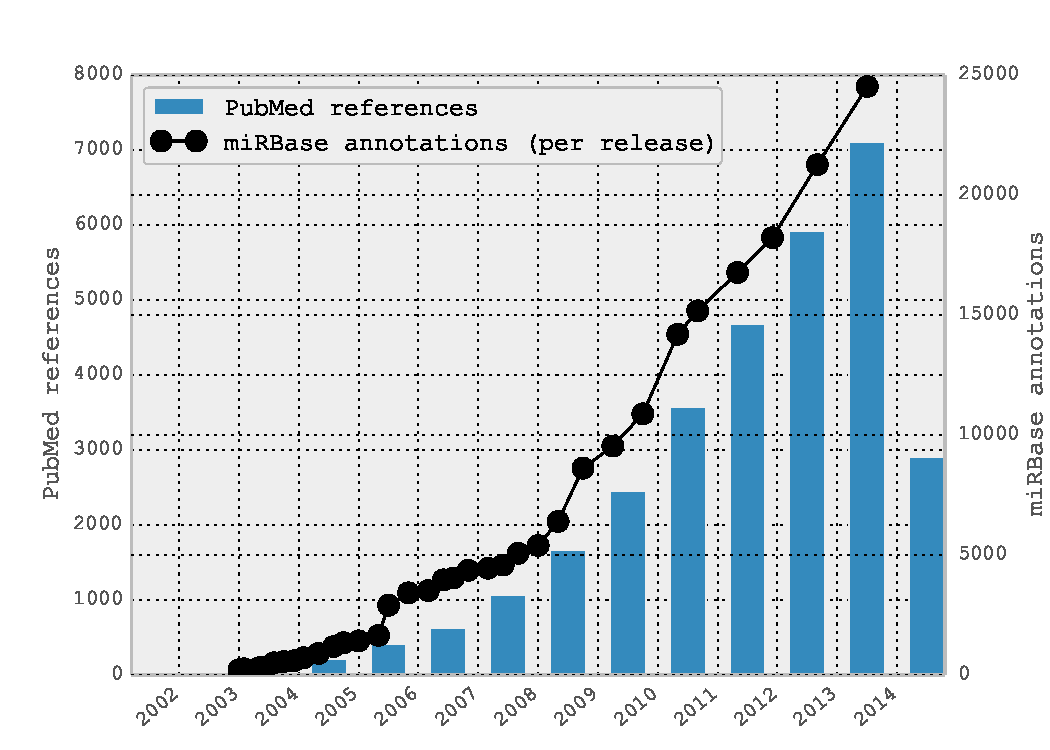
\includegraphics[width=\textwidth,natwidth=100,natheight=100]{image/mirna_history.pdf}
      \caption{The miRBase miRNA annotation collection has grown with the scientific community's interest in miRNAs. (Sources: http://www.mirbase.org/, http://www.ncbi.nlm.nih.gov/pubmed)}
      \label{fig:mirna_history}
\end{figure}

The characteristic biogenesis pathways of this group of ncRNA lead to the definition of the term microRNA in order to distinguish these transcripts from simliar-sized siRNA. In the canonical biogenesis pathway, mature (single stranded, $\sim22$-nt RNA molecules) miRNA are transcribed and subsequently processed through a variety of proteins. After transcription, primary miRNA is cleaved by the Drosha-DGCR8 complex into hairpin-shaped precursor-miRNA. These hairpins are exported into the cytosol by Exportin-5, through which the endonuclease Dicer cleaves the hairpins into $\sim~22$-nt duplexes. After the two strands separate one is loaded into the RNA-Induced Silencing Complex (RISC), through with miRNA exercise their regulatory functions. Among all the steps in this pathway, Exportin-5 and Dicer depend on the length of the miRNA.

The main function of miRNA is to target and suppress the translation of mRNA transcripts through either destroying the mRNA transcript or inhibiting mRNA translation. Typically, miRNA suppress gene expression through increasing the degradation rate of mRNA transcripts (referred to as mRNA destabilisation). In most cases, miRNA bind to the 3' UTR of mRNA transcripts, although exceptions have been reported. The deciding factor in the target selection has been the miRNA seed region, bases 1 through 8 at the 5' end of the mature miRNA. Imperfect binding in the seed region can be compensated by sequence complementarity in the remain gin part of the mature miRNA. In plants, perfect Watson-Crick base-pairing for the mature miRNA is required for translational inhibition.


\section{Methods}\label{method}

All code underlying this work is available at \url{https://github.com/davetang/mirna_length}. Briefly, random sequences were generated using R (version 3.1.0) and the R Bioconductor package Biostrings\cite{biostrings_package}. We generated three sets of one million random sequences that ranged from 15 to 30 base pairs in length, totalling 48 million sequences. The first two sets of sequences were generated based on the multinomial sequence model where each nucleotide in the sequence is independent and identically distributed based on a probability. The first set of randomly generated sequences used an equal probability for each nucleotide ($p_{a} = 0.25$, $p_{c} = 0.25$, $p_{g} = 0.25$, $p_{t} = 0.25$) and the second set used probabilities based on the nucleotide frequency observed in the human genome (hg38): $p_{a} = 0.29$, $p_{c} = 0.20$, $p_{g} = 0.21$, $p_{t} = 0.30$. The third set of randomly generated sequences used a Markov chain model, where the next sequence depends on the previous sequence. Transitions probabilities (Figure ~\ref{fig:transition}) were derived from the dinucleotide frequencies observed from a set of mature human miRNAs downloaded from miRBase\cite{pmid21037258}. The probability of the first base was derived from the frequency of nucleotides at the first base of human mature miRNAs. The alignment of the sequences was performed using BWA\cite{pmid19451168} (version 0.7.9a-r786) using aln/samse and summaries of the mapping were created using Perl scripts. The bar plots were created in R using ggplot2\cite{ggplot2_book} and reshape2\cite{reshape_wickham}.

\begin{figure}[t]
   \centering
   \begin{subfigure}{.5\textwidth}
      \centering
      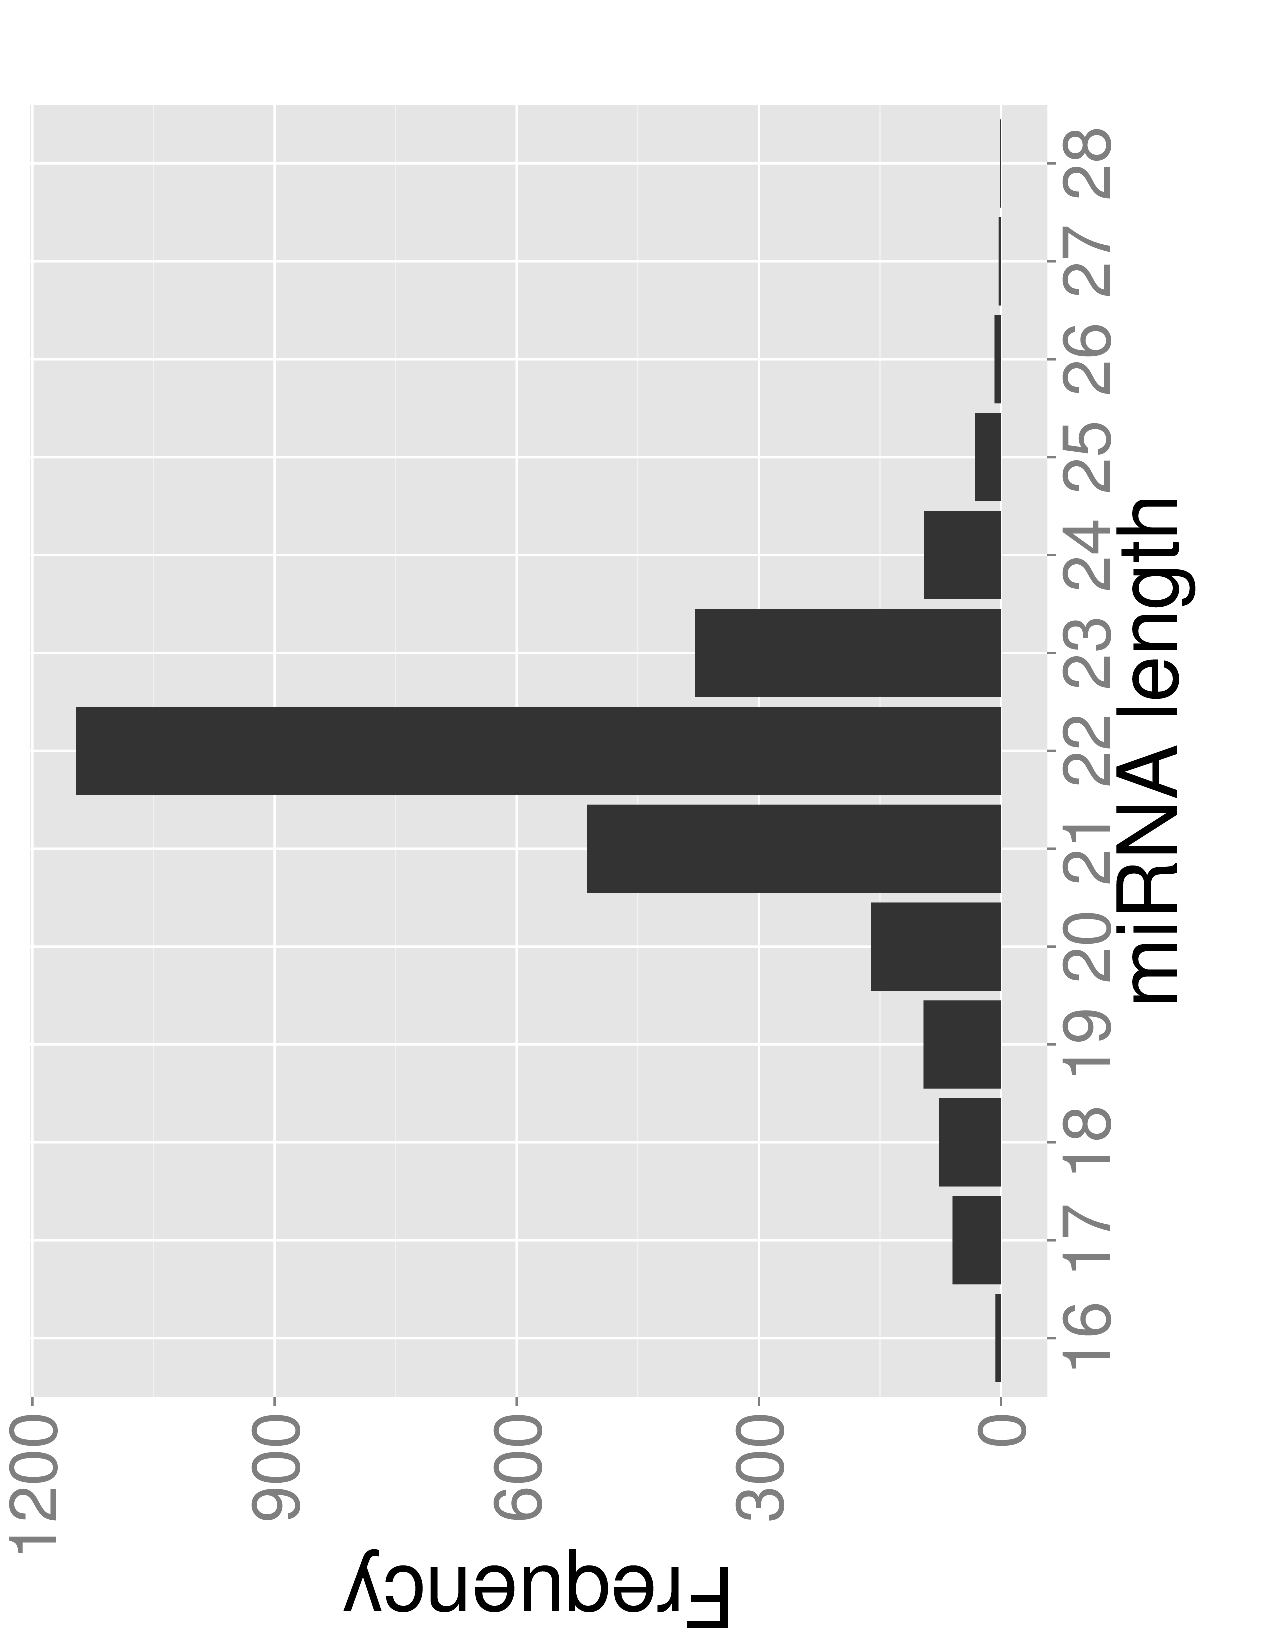
\includegraphics[width=.7\textwidth,natwidth=100,natheight=100,angle=270]{human_mirbase_length.pdf}
      \caption{}
      \label{fig:human_mirna_length}
   \end{subfigure}%
   \begin{subfigure}{.5\textwidth}
      \centering
      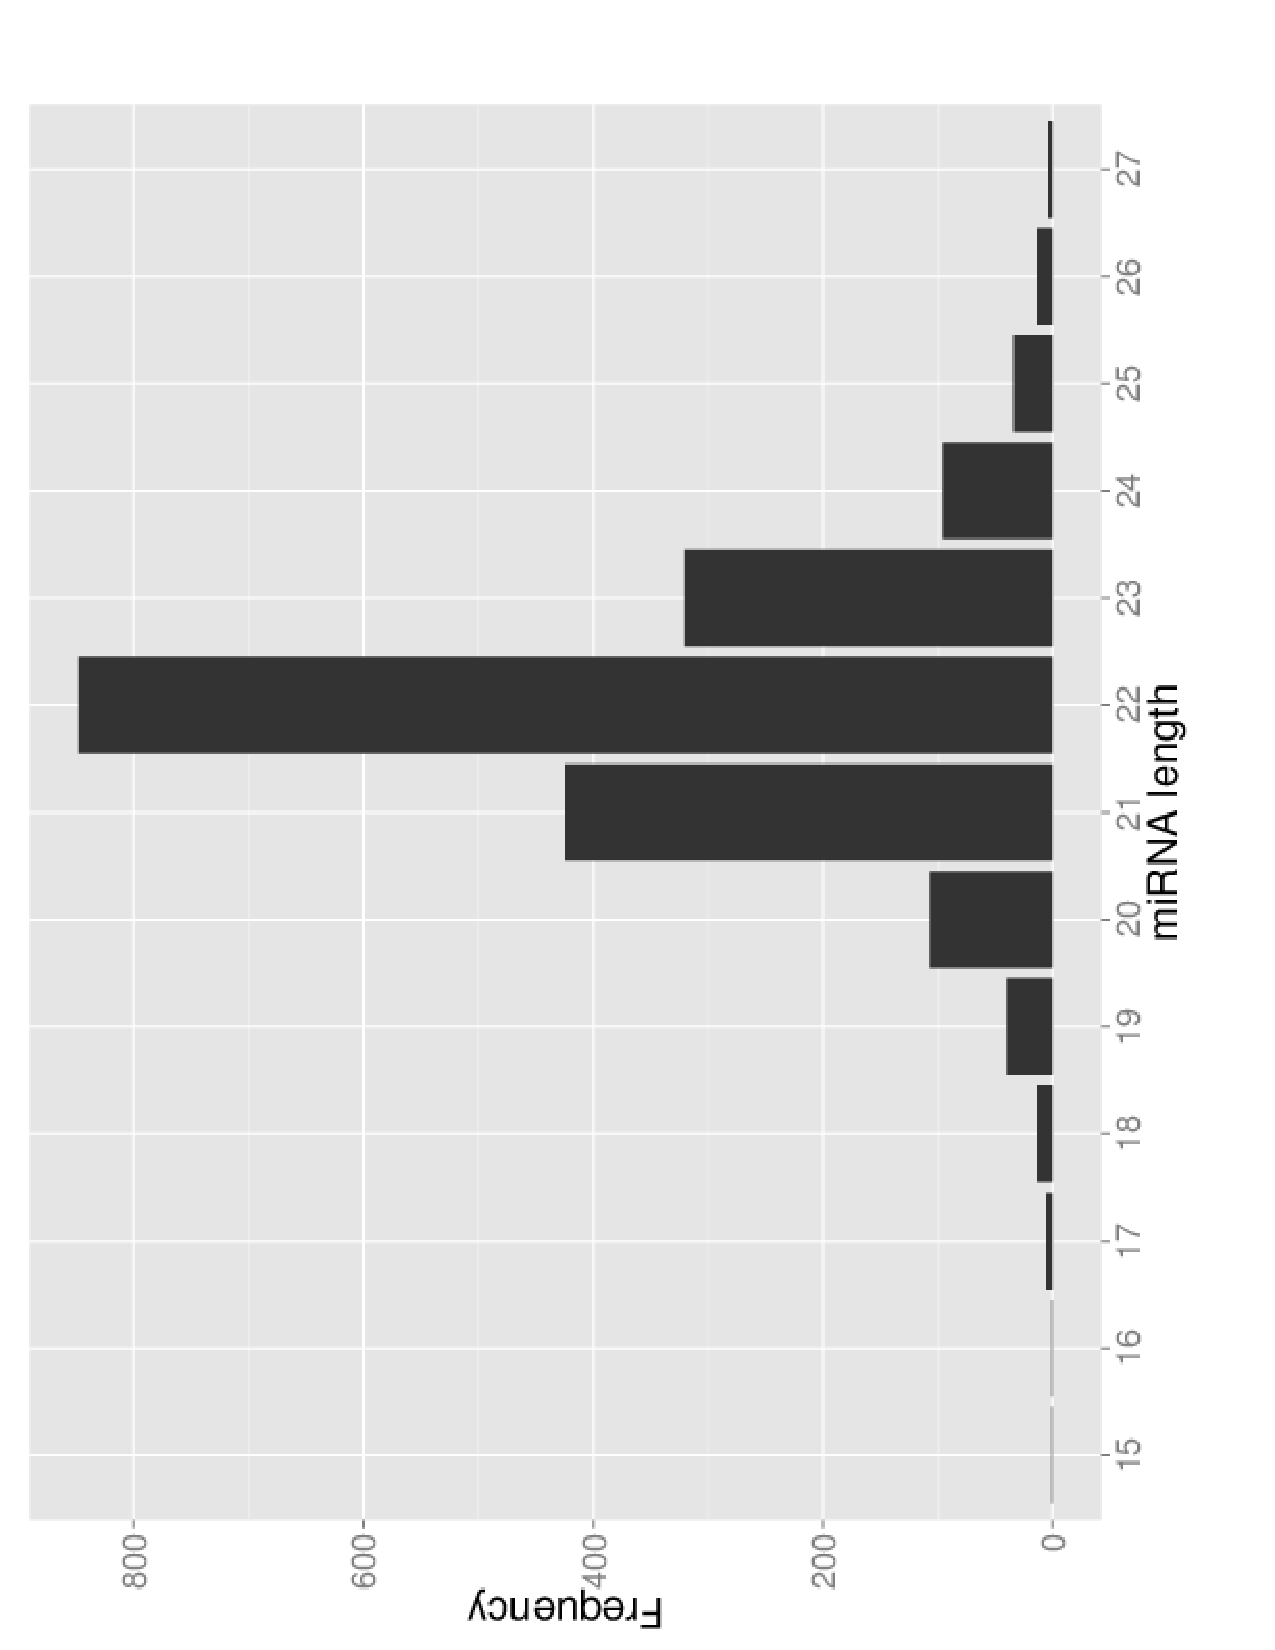
\includegraphics[width=.7\textwidth,natwidth=100,natheight=100,angle=270]{mouse_mirbase_length.pdf}
      \caption{}
      \label{fig:mouse_mirna_length}
   \end{subfigure}
   \begin{subfigure}{.5\columnwidth}
      \centering
      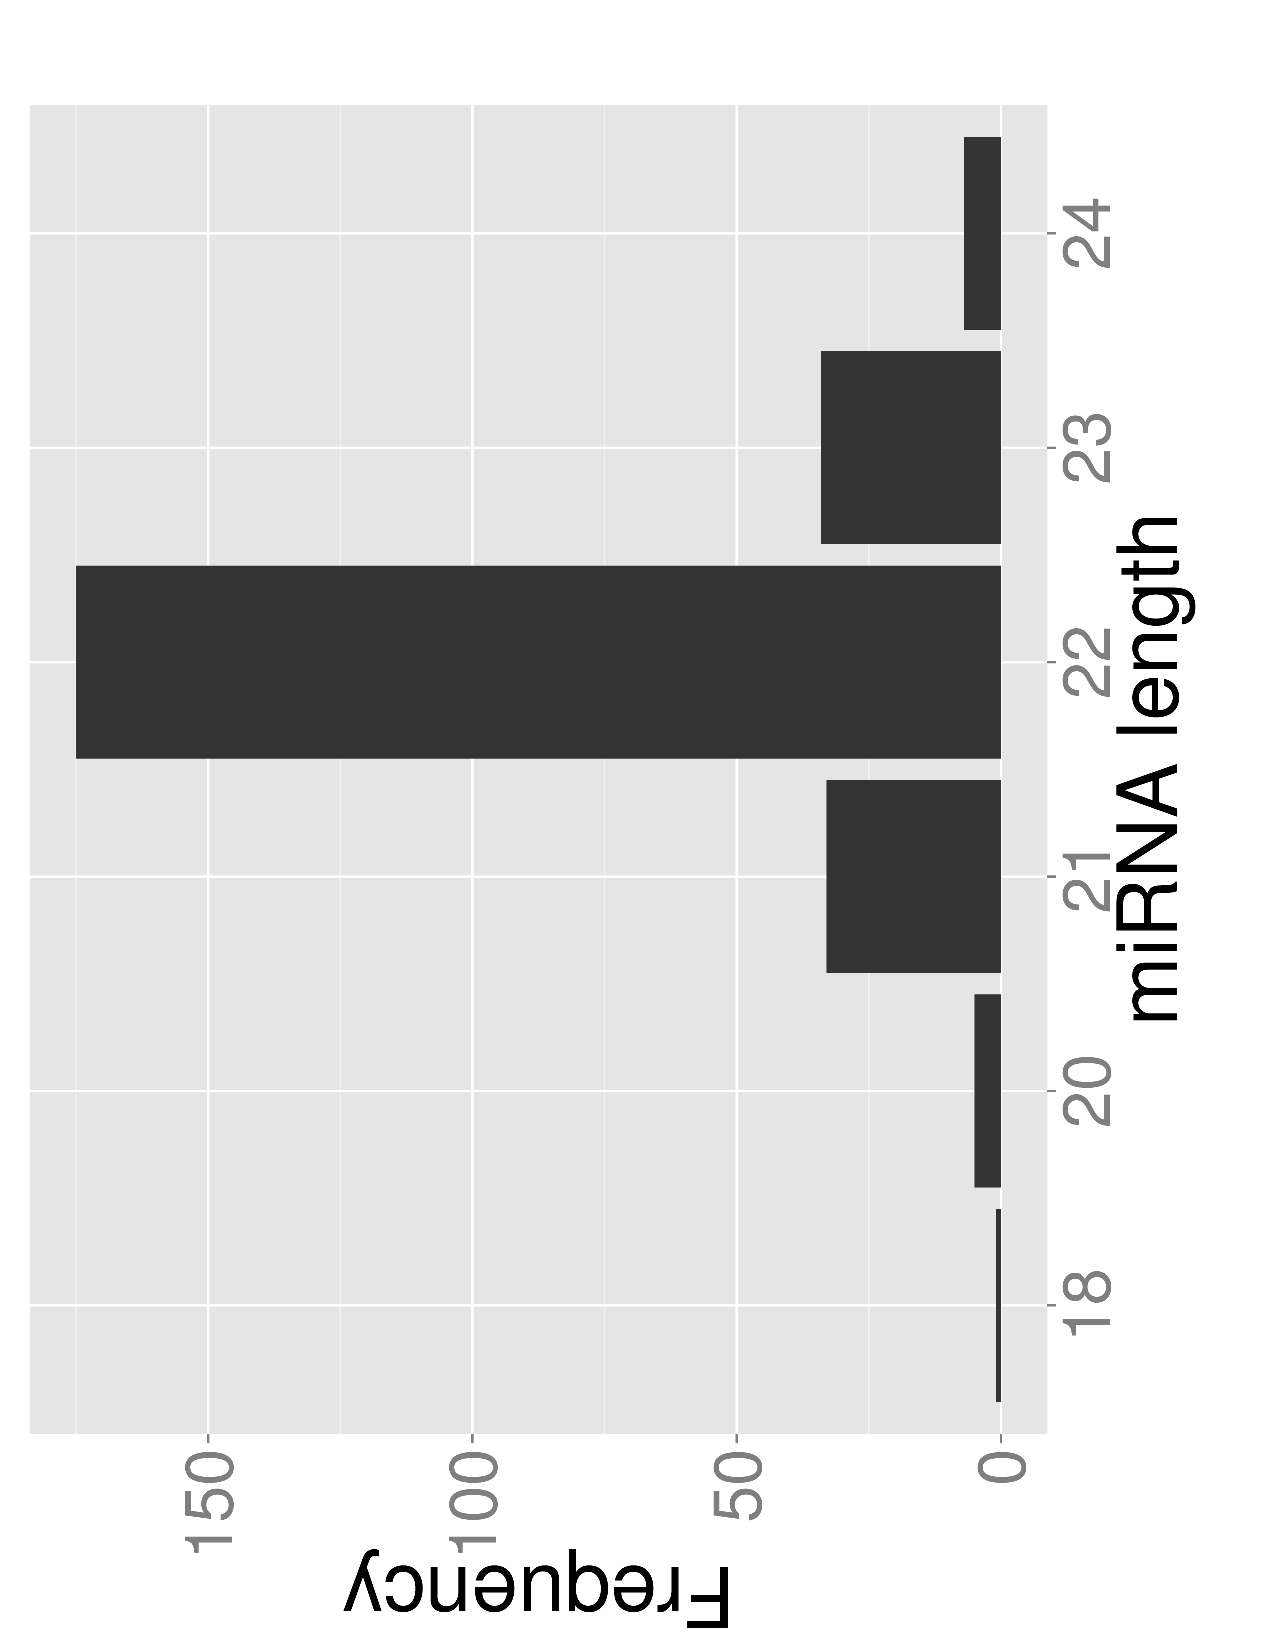
\includegraphics[width=.7\textwidth,natwidth=100,natheight=100,angle=270]{zebrafish_mirbase_length.pdf}
      \caption{}
      \label{fig:zebrafish_mirna_length}
   \end{subfigure}%
   \begin{subfigure}{.5\columnwidth}
      \centering
      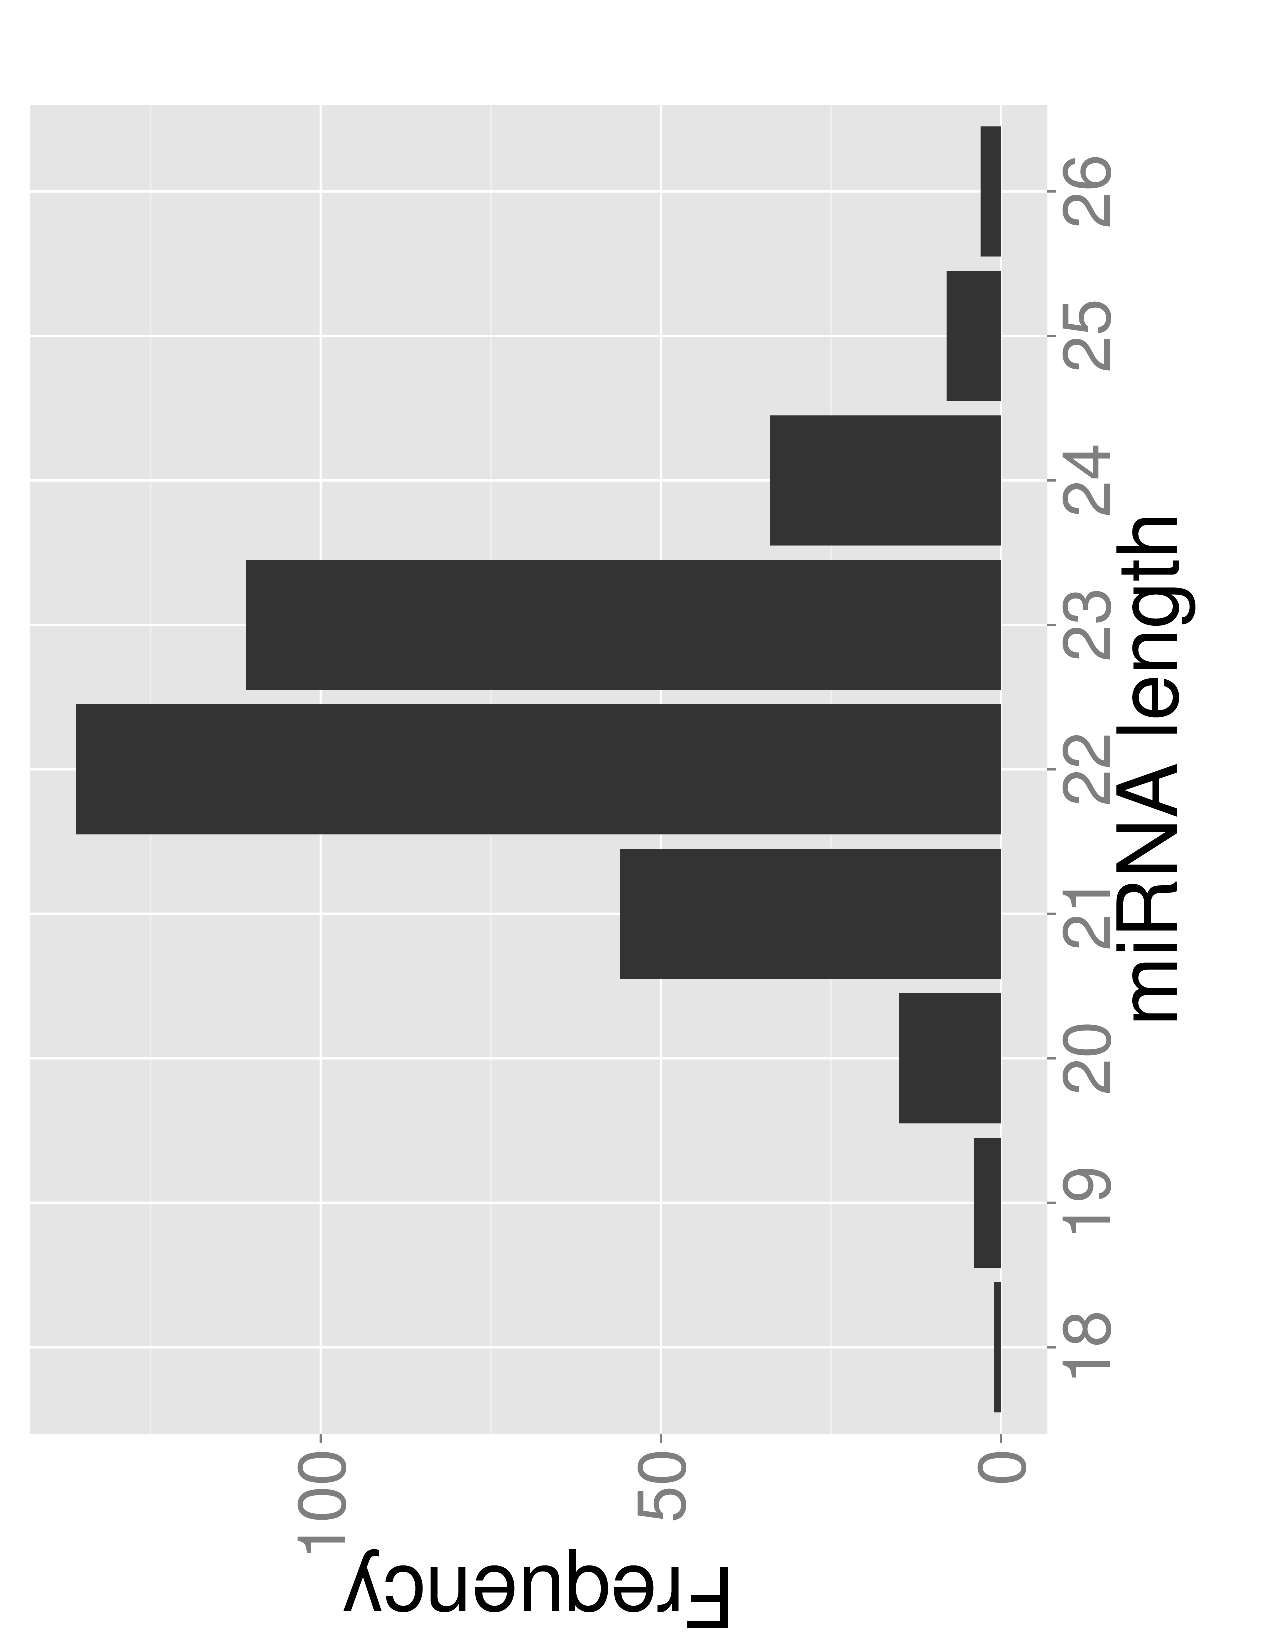
\includegraphics[width=.7\textwidth,natwidth=100,natheight=100,angle=270]{celegans_mirbase_length.pdf}
      \caption{}
      \label{fig:celegans_mirna_length}
   \end{subfigure}
   \caption{Length of miRNAs from miRBase for (a) human, (b) mouse, (c) zebrafish, and (d) nematode.}
   \label{fig:mirna_length}
\end{figure}

\begin{figure}[t]
   \centering
   \begin{subfigure}{.5\textwidth}
      \centering
      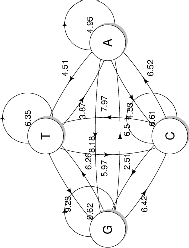
\includegraphics[width=.7\textwidth,natwidth=100,natheight=100,angle=270]{hg38.pdf}
      \caption{}
      \label{fig:hg38_transition}
   \end{subfigure}%
   \begin{subfigure}{.5\textwidth}
      \centering
      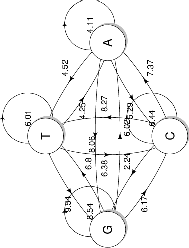
\includegraphics[width=.7\textwidth,natwidth=100,natheight=100,angle=270]{mm10.pdf}
      \caption{}
      \label{fig:mm10_transition}
   \end{subfigure}
   \begin{subfigure}{.5\columnwidth}
      \centering
      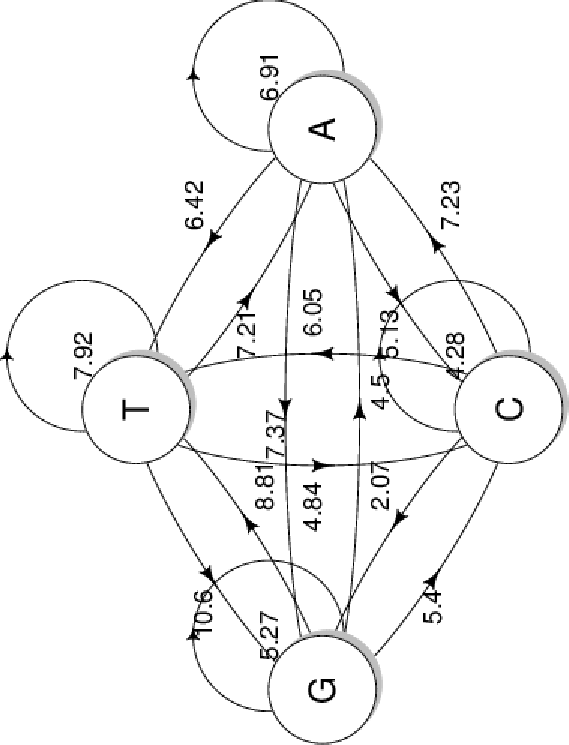
\includegraphics[width=.7\textwidth,natwidth=100,natheight=100,angle=270]{danRer7.pdf}
      \caption{}
      \label{fig:danRer7_transition}
   \end{subfigure}%
   \begin{subfigure}{.5\columnwidth}
      \centering
      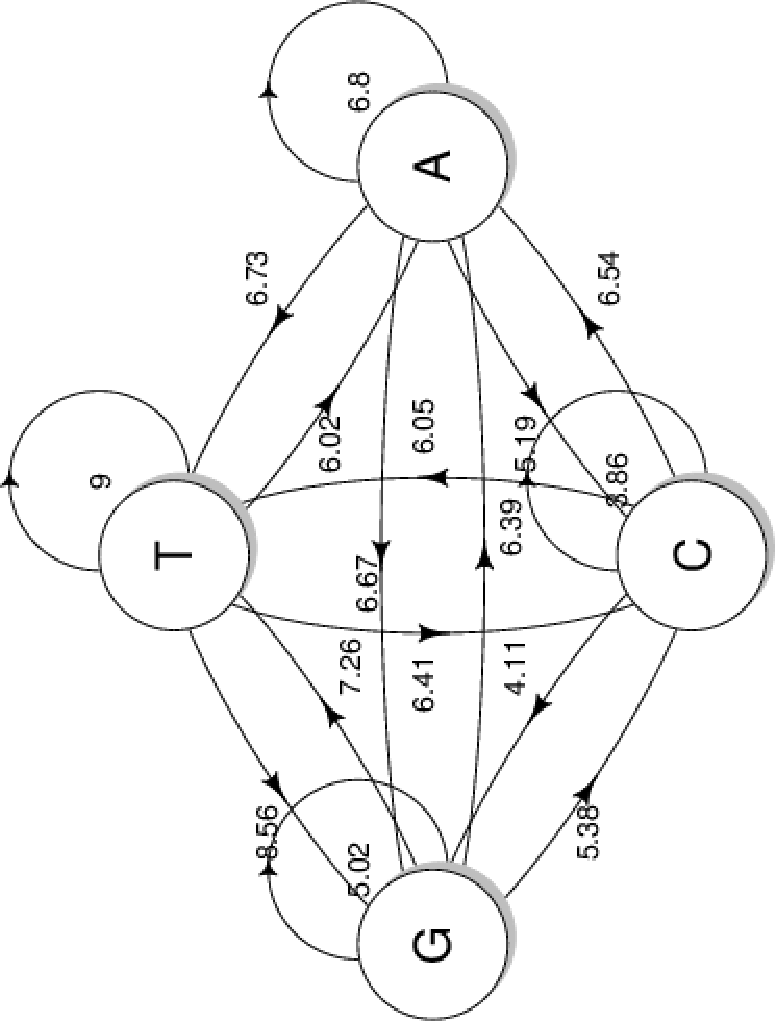
\includegraphics[width=.7\textwidth,natwidth=100,natheight=100,angle=270]{ce10.pdf}
      \caption{}
      \label{fig:ce10_transition}
   \end{subfigure}
   \caption{Transition diagrams for (a) human, (b) mouse, (c) zebrafish, and (d) nematode based on dinucleotide frequencies from miRBase mature miRNAs.}
   \label{fig:transition}
\end{figure}

\section{Results}\label{result}

The human genome is mainly composed of repetitive elements, many of which are transposable elements and thus its sequence composition is not a mosaic of random sequences. With this in mind, we would expect that randomly generated sequences would not map back to the human genome. However, it is not known at what length, random sequences will not map back. We investigated this by generating random sequences ranging from 15 base pairs to 30 base pairs under three different models (Section ~\ref{method}) and mapped these sequences to the human genome (Figure ~\ref{fig:mapped_statistic}a). At length 18, almost all randomly generated sequences could be mapped to the genome. The number of possible DNA sequences of \textit{n} length is $4^{n}$ and thus a 18 base pair sequence has 68,719,476,736 possible sequences.

\begin{figure}[t]
   \centering
   \begin{subfigure}{.5\textwidth}
      \centering
      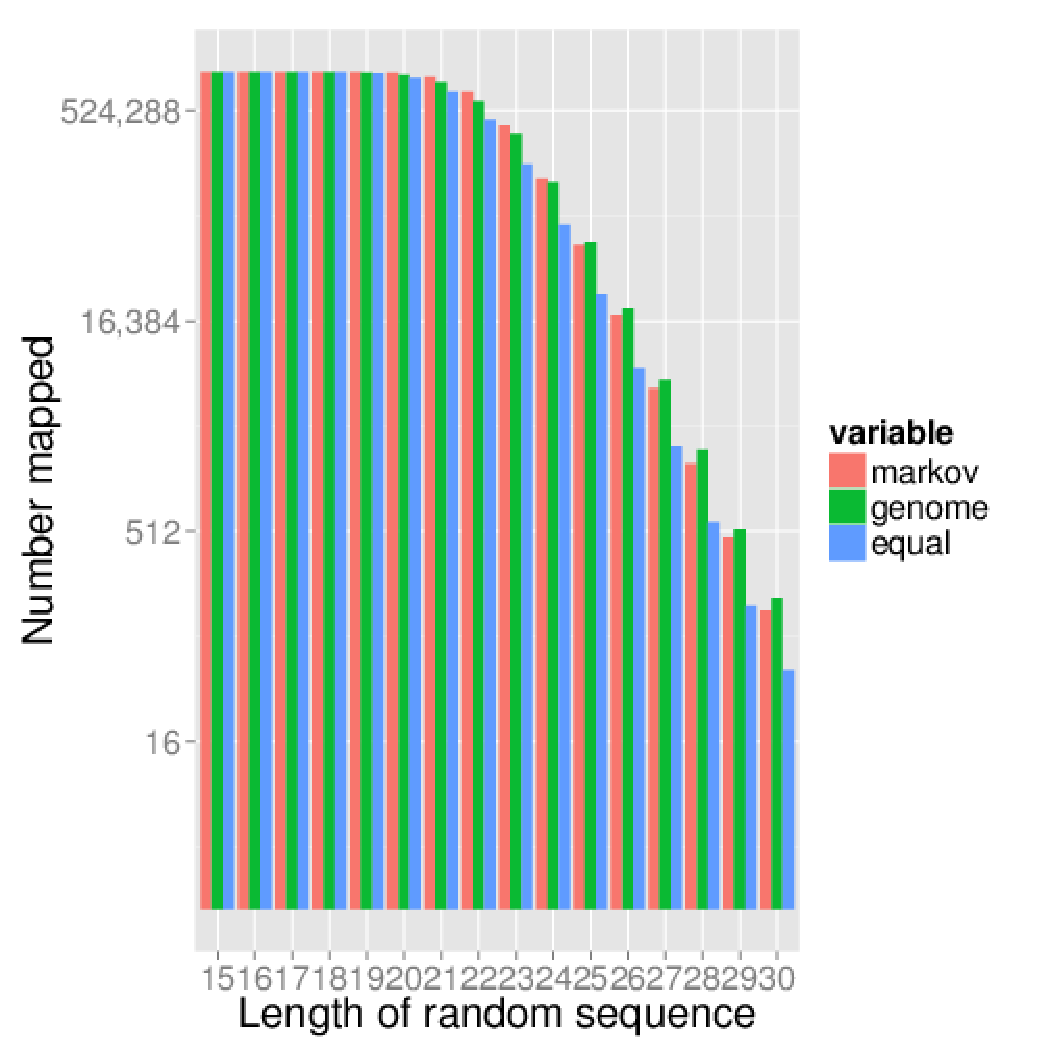
\includegraphics[width=.9\textwidth,natwidth=100,natheight=100]{hg38_mapped_1000000.pdf}
      \caption{}
      \label{fig:hg38_mapped}
   \end{subfigure}%
   \begin{subfigure}{.5\textwidth}
      \centering
      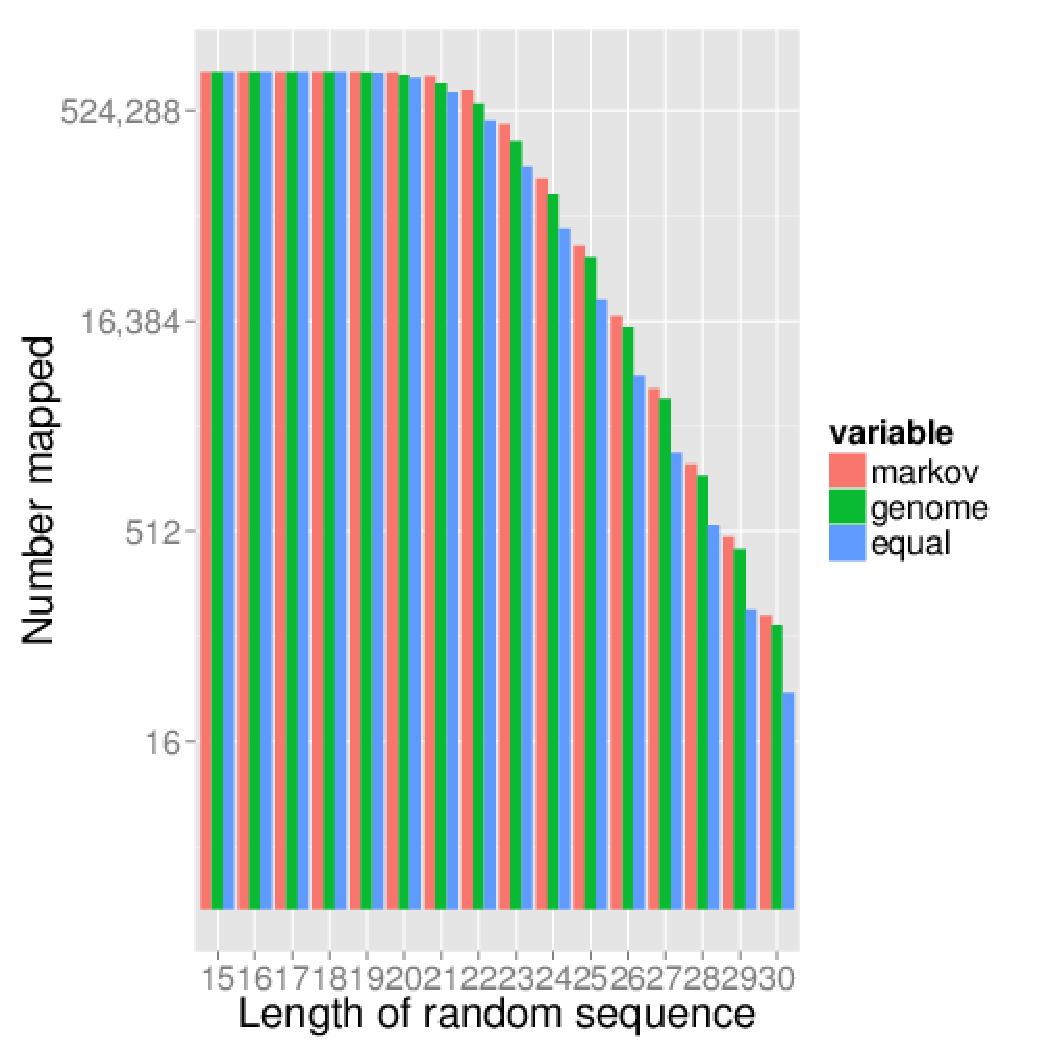
\includegraphics[width=.9\textwidth,natwidth=100,natheight=100]{mm10_mapped_1000000.pdf}
      \caption{}
      \label{fig:mm10_mapped}
   \end{subfigure}
   \begin{subfigure}{.5\columnwidth}
      \centering
      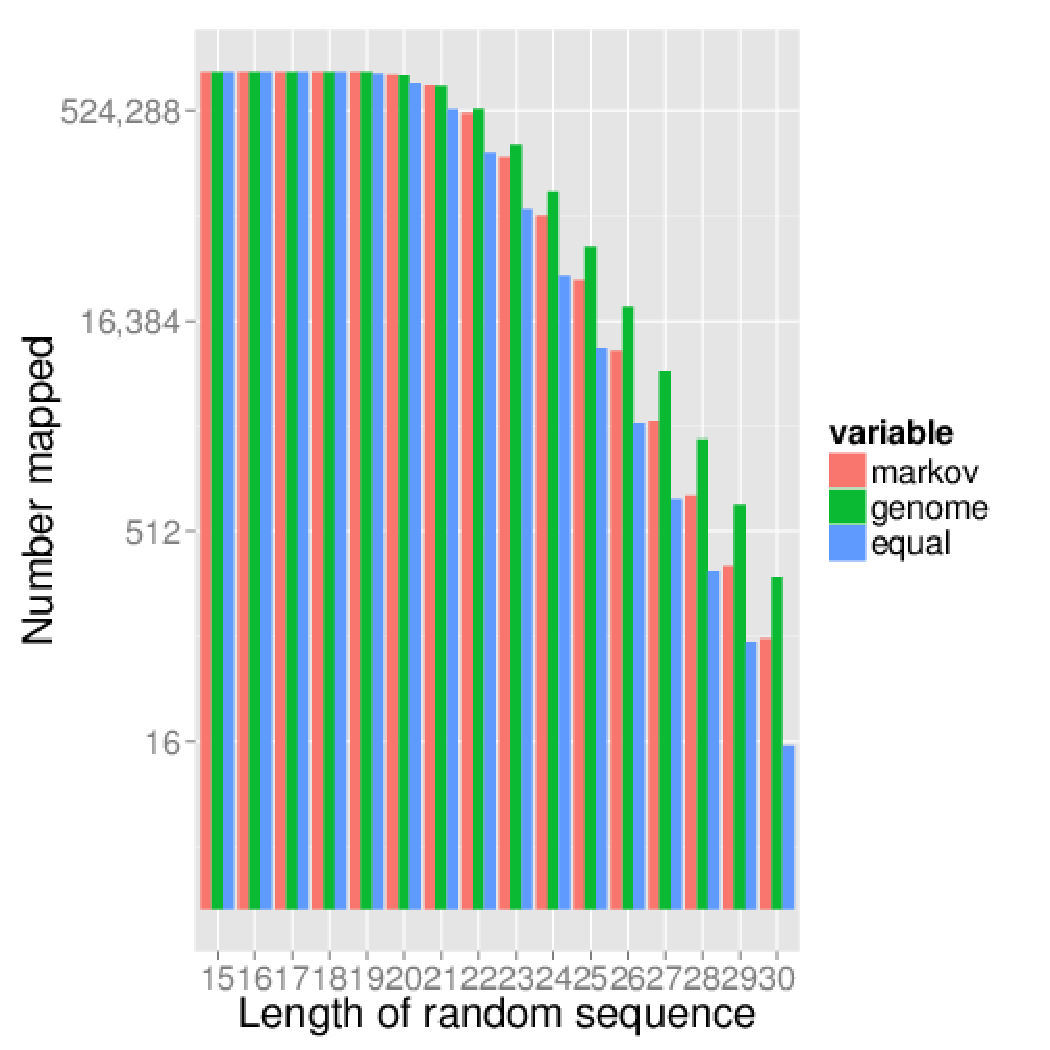
\includegraphics[width=.9\textwidth,natwidth=100,natheight=100]{danRer7_mapped_1000000.pdf}
      \caption{}
      \label{fig:danRer7_mapped}
   \end{subfigure}%
   \begin{subfigure}{.5\columnwidth}
      \centering
      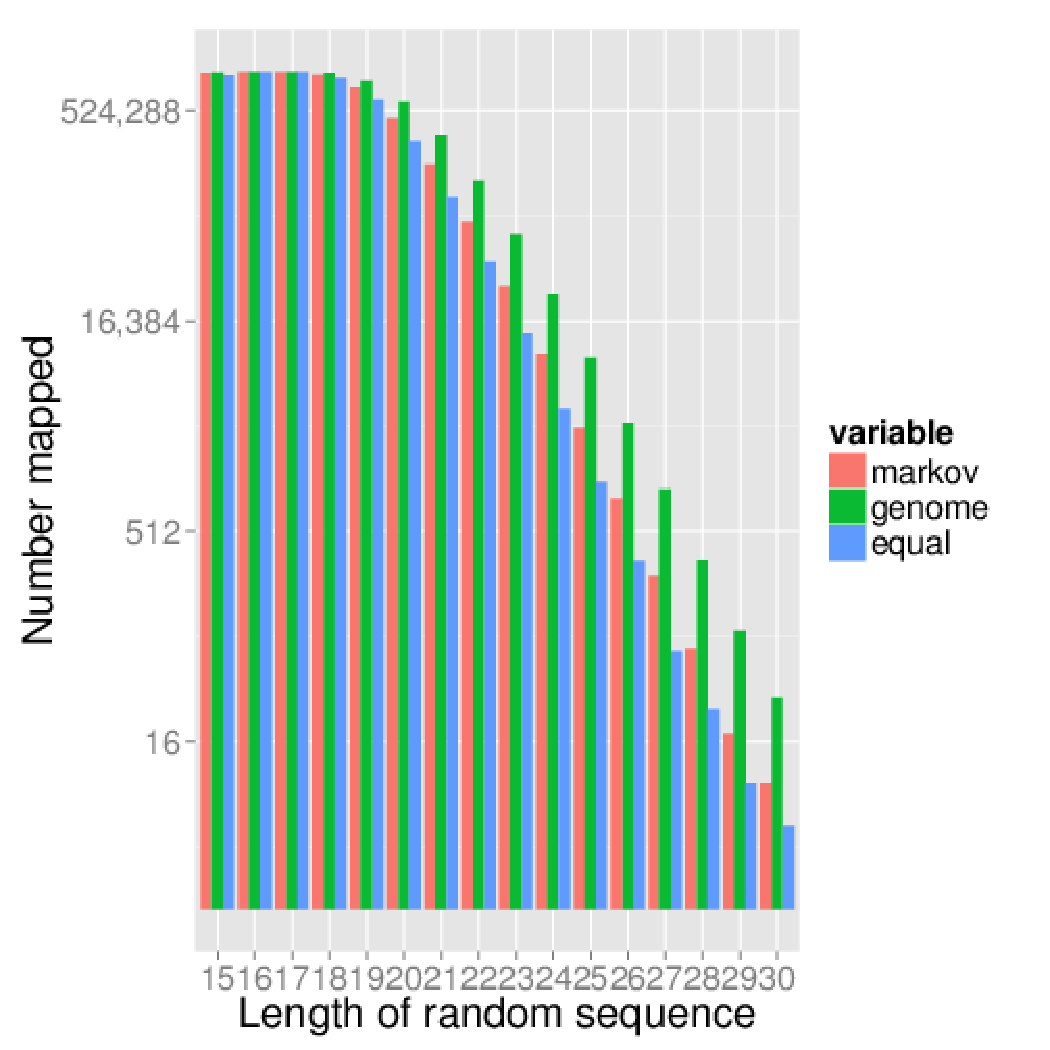
\includegraphics[width=.9\textwidth,natwidth=100,natheight=100]{ce10_mapped_1000000.pdf}
      \caption{}
      \label{fig:ce10_mapped}
   \end{subfigure}
   \caption{}
   \label{fig:mapped_statistic}
\end{figure}

\blindtext

\begin{figure}[t]
   \centering
   \begin{subfigure}{.5\textwidth}
      \centering
      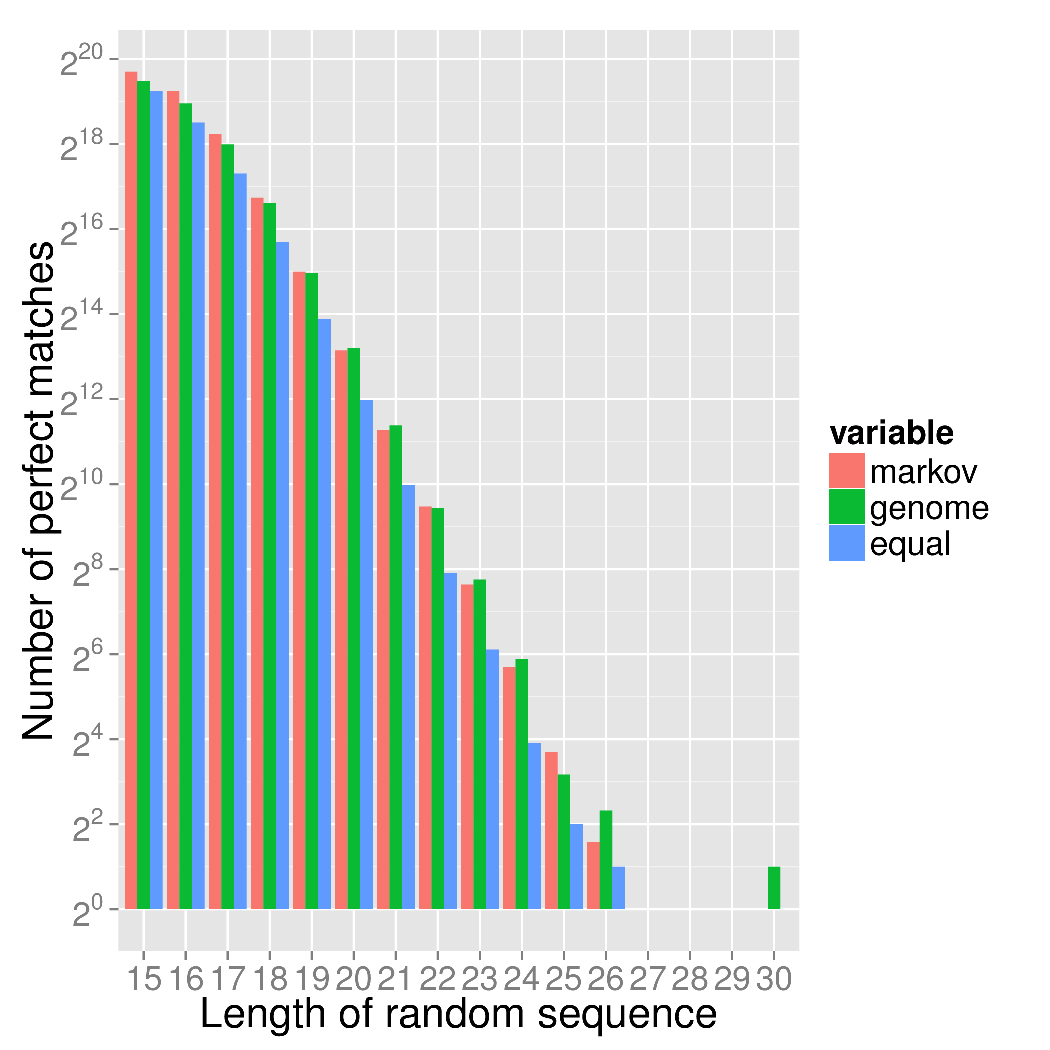
\includegraphics[width=.9\textwidth,natwidth=100,natheight=100]{hg38_perfect_mapped_1000000.pdf}
      \caption{}
      \label{fig:hg38_mapped_perfect}
   \end{subfigure}%
   \begin{subfigure}{.5\textwidth}
      \centering
      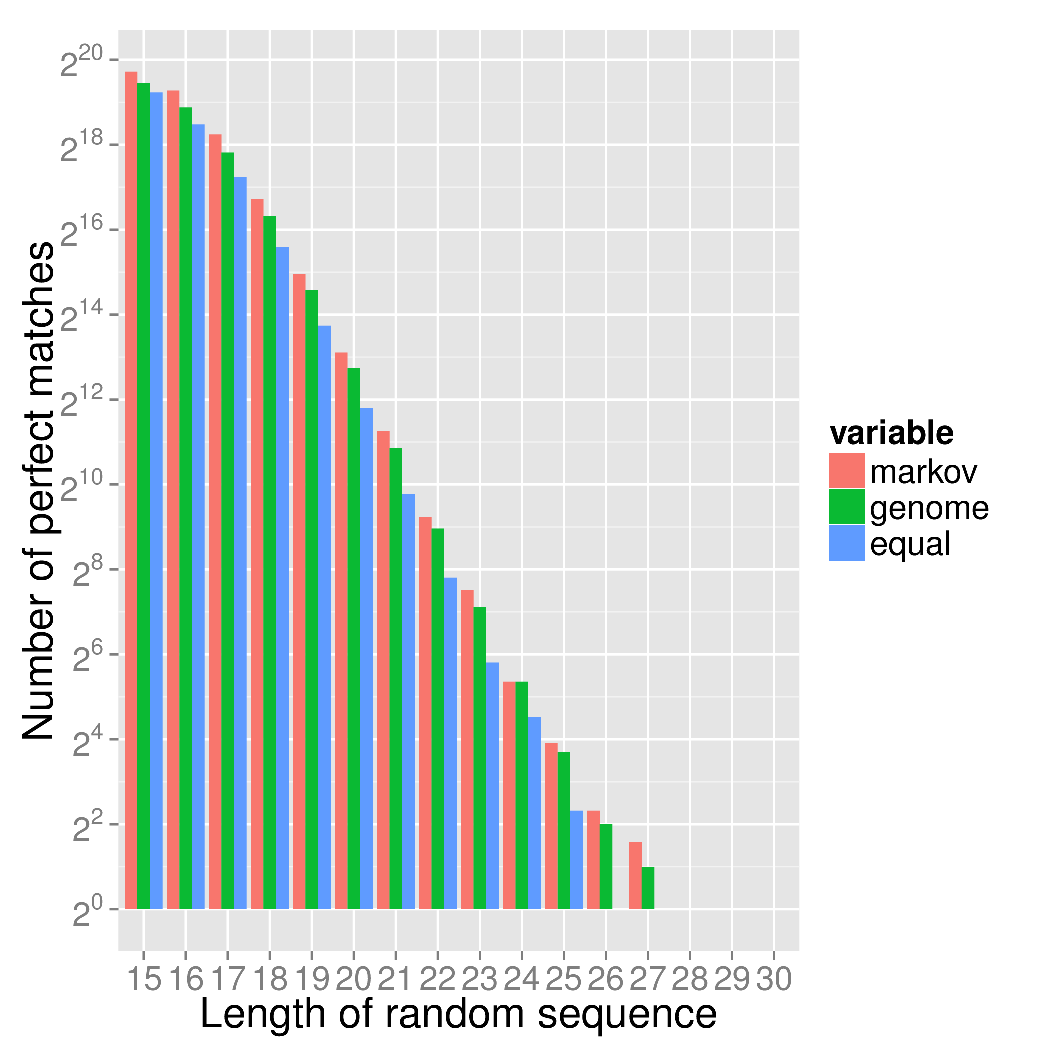
\includegraphics[width=.9\textwidth,natwidth=100,natheight=100]{mm10_perfect_mapped_1000000.pdf}
      \caption{}
      \label{fig:mm10_mapped_perfect}
   \end{subfigure}  
   \begin{subfigure}{.5\columnwidth}
      \centering
      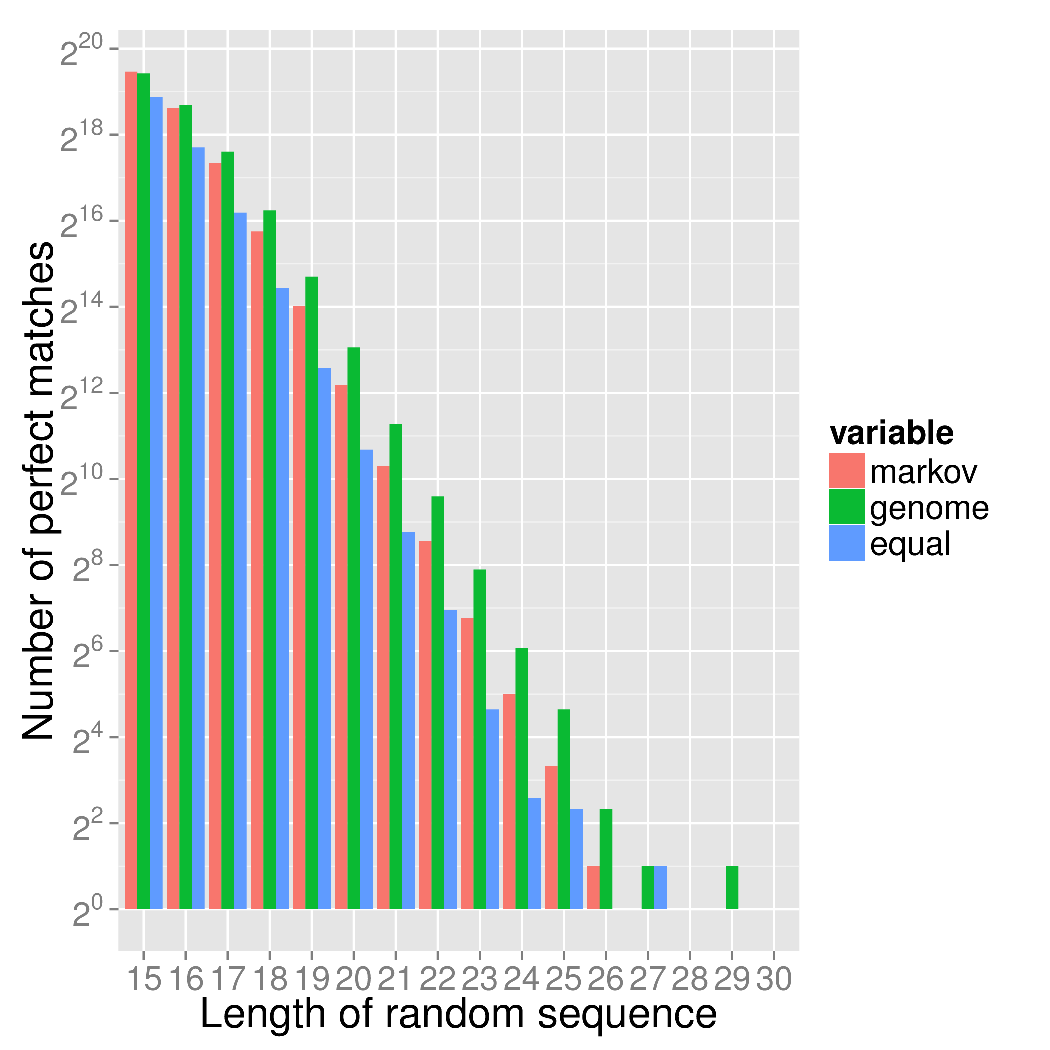
\includegraphics[width=.9\textwidth,natwidth=100,natheight=100]{danRer7_perfect_mapped_1000000.pdf}
      \caption{}
      \label{fig:danRer7_mapped_perfect}
   \end{subfigure}%
   \begin{subfigure}{.5\columnwidth}
      \centering
      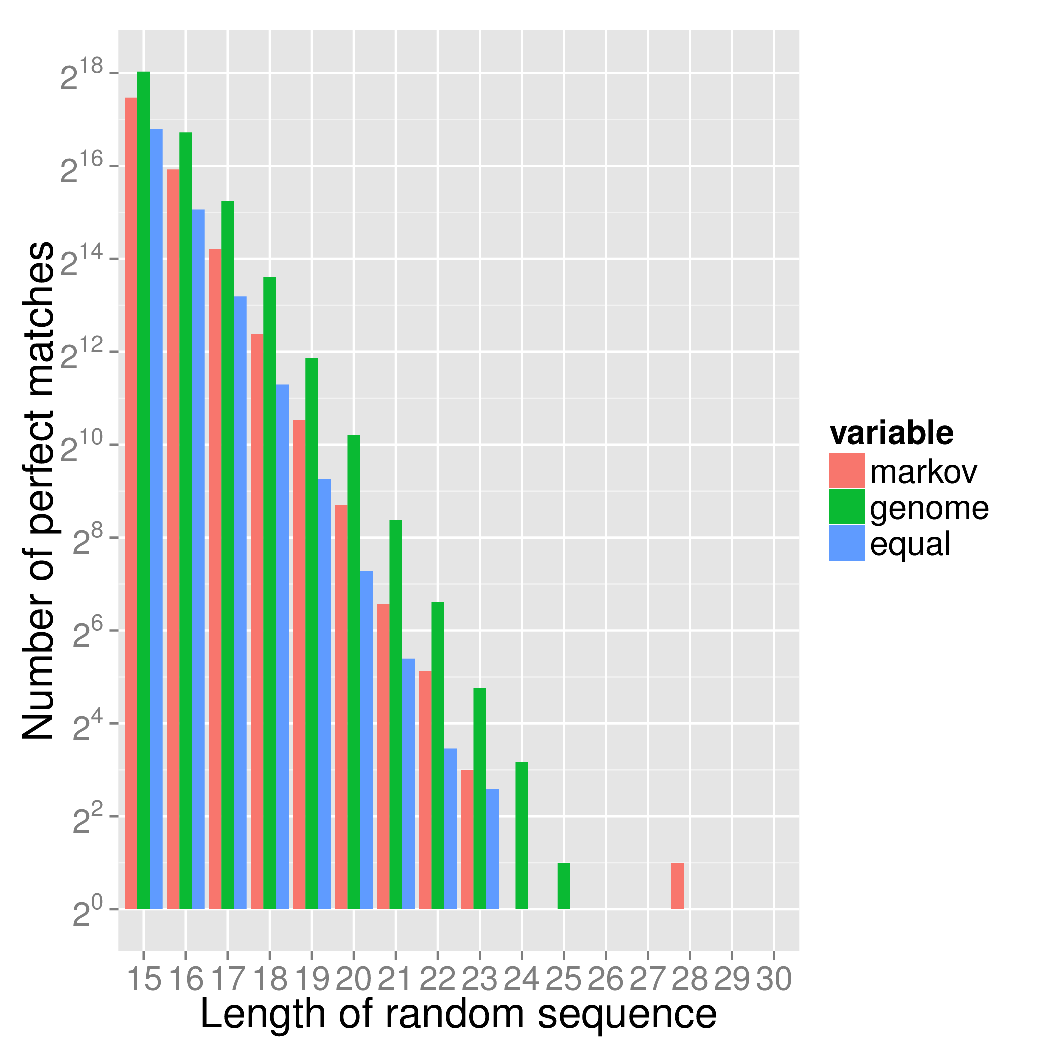
\includegraphics[width=.9\textwidth,natwidth=100,natheight=100]{ce10_perfect_mapped_1000000.pdf}
      \caption{}
      \label{fig:ce10_mapped_perfect}
   \end{subfigure}
   \caption{}
   \label{fig:mapped_perfect_statistic}
\end{figure}

\section{Discussion}\label{discussion}

Mammalian miRNAs are able to recognise their target miRNA by as little as 6-8 nucleotides; this region is known as the seed region, which lies at the 5' end of a miRNA. However despite this, most miRNAs are 22-23 base pairs in length.

\section{Authors' contributions}

DD wrote the section on miRNAs, suggested analyses, and discussed the results. DT did everything else. All authors read and approved the final manuscript.

\newpage

\bibliographystyle{unsrt}
\bibliography{ref}

\end{document}
